\section{First prototype}\label{ch:first_prototype}

The prototype model has to be able to classify and to localize \name{nodes} and \name{constraints}; whereas \name{constraints} are connecting pairs of \name{nodes} respectively.
Classification is the problem of detecting the correct type of \name{nodes} or \name{constraints}. % TODO citation
Localization is the problem of determining the position of the respective detection inside of a given image. % TODO citation
Subsequently, the gathered information has to be transformed into a usable format for further processing, e.g.\ into JSON to be usable by \name{mec2}. % TODO citation needed?

\subsection{The Fully Convolutional Network}\label{ch:fcn}

The topic of prepending work was the classification of hand-drawn mechanical symbols~\cite{Lawrence2020}.
The resulting model can classify images with size 32 by 32 pixels as \name{nodes}, \name{base-nodes} or neither of both.
It is only capable of classifying images with exactly these dimensions, which is insufficient for the task at hand.
However, the model can be extended to be able to provide not only a classification, but also the location of an element in an image of arbitrary size.

To examine the model it can be loaded using \name{Keras'}, % TODO citation should be in the introduction.
\code{model.load\_model} function and by issuing the \code{summary} method we get Listing~\ref{lst:srp_model}.

\begin{lstlisting}[caption={Summary of Symbol Classifier.}, label={lst:srp_model}]
_________________________________________________________________
Layer (type)                 Output Shape              Param #
=================================================================
conv2d (Conv2D)              (None, 32, 32, 16)        272
_________________________________________________________________
max_pooling2d (MaxPooling2D) (None, 16, 16, 16)        0
_________________________________________________________________
conv2d_1 (Conv2D)            (None, 16, 16, 32)        8224
_________________________________________________________________
max_pooling2d_1 (MaxPooling2 (None, 8, 8, 32)          0
_________________________________________________________________
flatten (Flatten)            (None, 2048)              0
_________________________________________________________________
dense (Dense)                (None, 3)                 6147
=================================================================
Total params: 14,643
Trainable params: 14,643
Non-trainable params: 0
_________________________________________________________________
\end{lstlisting}

The naive way to localize detected \name{nodes} and \name{constraints} in an image of arbitrary size is to scan sectors of size 32 by 32 pixels of an image and predicting them individually.
Using a 360\times360 sized image with strides of one in each direction, the number of images which are used in the prediction process are 108.241 images\footnote{\(h + 1 - 32 * w + 1 - 32\), where \(h\) and \(w\) are the height and width of the input image and the size of the kernel used to predict is 32}.
The respective Jupyter notebook testing the performance of this method can be reviewed at \url{https://aka.klawr.de/sep#1}. % TODO Set this URL.

To test this amount of images is not necessary most of the time and can be reduced by increasing the stride of the respective scanning process.
This would most likely reduce the accuracy of localizations, but would certainly increase the speed of the operation.

Another approach is to use the properties of convolutional layers to restructure the model and thereby making the whole procedure much more efficient.
To transform the model into a so-called Fully Convolutional Network (FCN) the input layer has to be prepended by a convolutional layer.
The first layer accepts images of arbitrary size.
The kernel of 32 by 32 determines the size of the segment given to the second layer, which was previously used as the input-layer.
Because the input of the original model is only defined by the kernel size, each successive layer is agnostic to the size of the previous.
Listing~\ref{lst:to_fcn} transforms the \code{old\_model} by appending an \code{tf.keras.Input} layer without any specified size and replacing the output layer by a \code{tf.keras.Conv2D} layer\footnote{And thus removing the \code{tf.keras.flatten} layer.}.

\begin{lstlisting}[caption={Transformation of the Symbol Classifier into a FCN.}, label=lst:to_fcn]
inputs = tf.keras.Input(shape=(None, None, 1))

hidden = old_model.layers[0](inputs)

for layer in old_model.layers[1:4]:
    hidden = layer(hidden)

# Get the input dimensions of the flattened layer:
f_dim = old_model.layers[4].input_shape
# And use it to convert the next dense layer:
dense = old_model.layers[5]
out_dim = dense.get_weights()[1].shape[0]
W, b = dense.get_weights()
new_W = W.reshape((f_dim[1], f_dim[2], f_dim[3], out_dim))
outputs = tf.keras.layers.Conv2D(out_dim,
                           (f_dim[1], f_dim[2]),
                           name = dense.name,
                           strides = (1, 1),
                           activation = dense.activation,
                           padding = 'valid',
                           weights = [new_W, b])(hidden)

model = tf.keras.Model(inputs = inputs, outputs = outputs)

model.summary()
\end{lstlisting}

An example of the usage of this code can be found at \url{https://aka.klawr.de/sep#2} % TODO
, where the intricate differences between both approaches are examined.

The FCN approach is roughly ten times faster than taking crops and predicting them individually. 
The \code{model.summary} results in the output given as Listing~\ref{lst:fcn_summary}:

\begin{lstlisting}[label={lst:fcn_summary}, caption={Summary of Symbol Classifier transformed into a FCN.}]
Model: "model"
_________________________________________________________________
Layer (type)                 Output Shape              Param #   
=================================================================
input_1 (InputLayer)         [(None, None, None, 1)]   0         
_________________________________________________________________
conv2d (Conv2D)              multiple                  272       
_________________________________________________________________
max_pooling2d (MaxPooling2D) multiple                  0         
_________________________________________________________________
conv2d_1 (Conv2D)            multiple                  8224      
_________________________________________________________________
max_pooling2d_1 (MaxPooling2 multiple                  0         
_________________________________________________________________
dense (Conv2D)               (None, None, None, 3)     6147      
=================================================================
Total params: 14,643
Trainable params: 14,643
Non-trainable params: 0
_________________________________________________________________
\end{lstlisting}

Granted the performance of this model is satisfactory for the moment, the problem of detecting constraints can be addressed.

\subsection{Constraint detection}

Besides a model to detect nodes, it is now necessary to train a model that can detect and classify constraints.
To create such a model suitable training data has to be generated first.

The model should be able to distinguish between two types of constraints:
Constraints to prevent nodes to change the range between each other, which allows only for rotational movement.
It is represented by an arrow with an arc at the origin.
The other type of constraint prevents motion that would change the angle between two nodes, which only allows translational movement between two nodes.
It is represented by an arrow with two gaps on the shaft and no arc at the origin.
Examples for the generated data can be seen in figure~\ref{fig:constraint_data}.

Furthermore, the data is split for constraints of different lengths.
This allows a better selection of a constraint when two nodes are to be connected when generating the training data.

Data generation for constraints is similar to data generation in~\cite{Lawrence2020}.
The drawing canvas has a width of fifty and the range can vary between 15--249, 250--349, or 350--449; depending on the selected range.

\begin{figure}
    \centering
    \begin{subfigure}[b]{0.45\textwidth}
        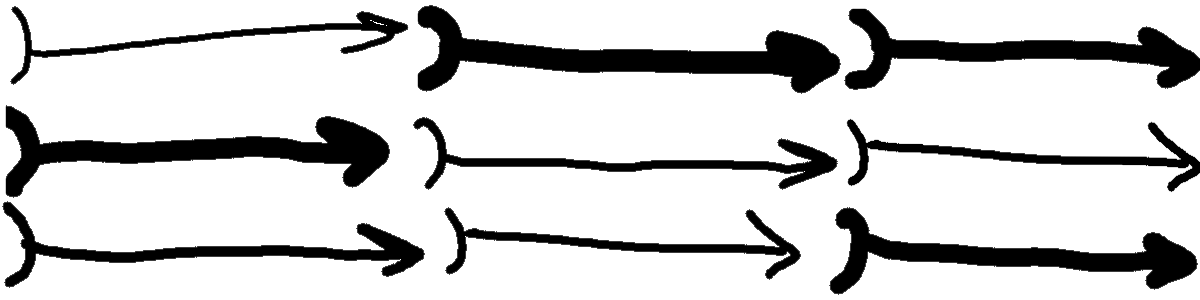
\includegraphics[width=\textwidth]{images/rs.png}
        \caption{Rotational Constraints}\label{fig:rotational_constraints}
    \end{subfigure}
    \begin{subfigure}[b]{0.45\textwidth}
        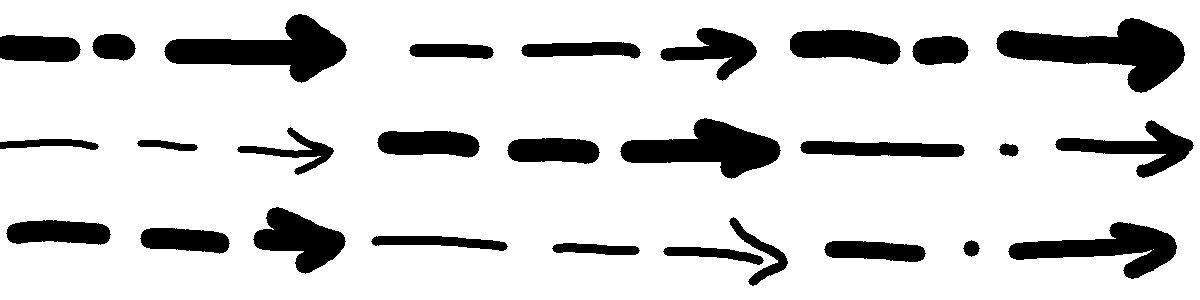
\includegraphics[width=\textwidth]{images/ts.png}
        \caption{Translational Constraints}\label{fig:translational_constraints}
    \end{subfigure}
    \caption[Examples of constraint detector training data]{Some examples of the data created with the described method. Only these two classes were created for the first tests. The images are created horizontally, so their initial angle can be assumed to be zero to keep a record when labeling the data dynamically. }\label{fig:constraint_data}
\end{figure}

For each type approximately 1200 images were drawn, 400 for each range, resulting in 2400 images. % TODO download link?
These images can be used with existing images of nodes to create realistic images of hand-drawn mechanisms.

\subsubsection{Preparing nodes on images}

Since constraints can occur at all possible angles, the data must be generated in such a way that it resembles real mechanisms best.
Because of this, multiple steps have to be taken to generate comprehensible training data.

Metadata generated during the generation process is saved into a format that is readable by \name{pandas}. % TODO citation needed
\name{pandas} is an open-source data analysis and manipulation tool which helps to work and to visualize data.

Each generated image begins with a black background of size 360\times360.
Between 3 and 10 nodes are randomly placed on the image\footnote{In an intermediate step the node data from previous work is modified to consist of white symbols on black background, instead of random grayscale images.}.
Each node has to have a minimum distance of 60 to every other node in the image.
Examples for the resulting images are shown in figure~\ref{fig:constraint_data_step1}.
The respective notebook containing the code for this process can be viewed at \url{https://aka.klawr.de/sep\#3}.
Using this method 100.000 images are generated.

\begin{figure}
    \centering
    \begin{subfigure}[b]{0.19\textwidth}
        \fbox{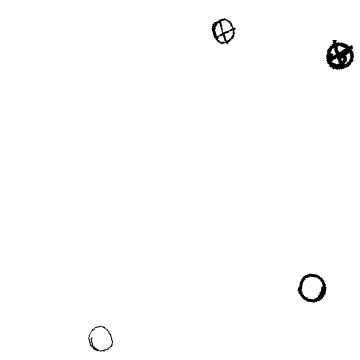
\includegraphics[width=0.92\textwidth]{images/1_0.png}}
    \end{subfigure}
    \begin{subfigure}[b]{0.19\textwidth}
        \fbox{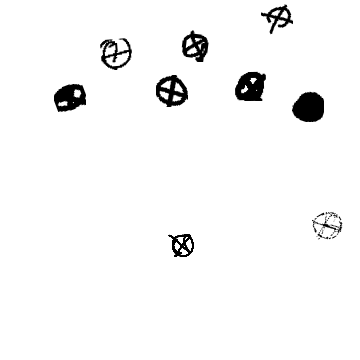
\includegraphics[width=0.92\textwidth]{images/1_1.png}}
    \end{subfigure}
    \begin{subfigure}[b]{0.19\textwidth}
        \fbox{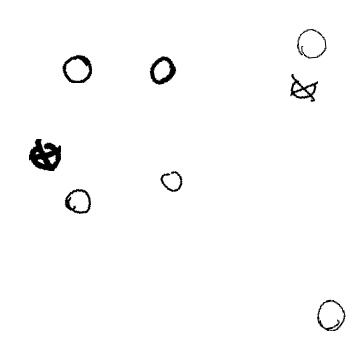
\includegraphics[width=0.92\textwidth]{images/1_2.png}}
    \end{subfigure}
    \begin{subfigure}[b]{0.19\textwidth}
        \fbox{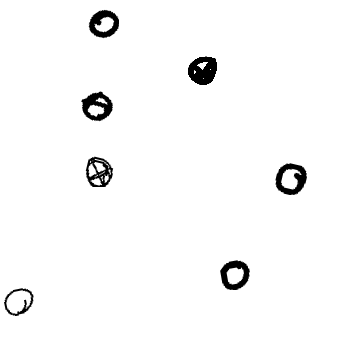
\includegraphics[width=0.92\textwidth]{images/1_3.png}}
    \end{subfigure}
    \begin{subfigure}[b]{0.19\textwidth}
        \fbox{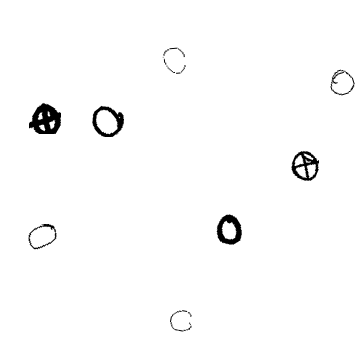
\includegraphics[width=0.92\textwidth]{images/1_4.png}}
    \end{subfigure}
    \caption[Randomly placed nodes on blank image]{Randomly placed nodes on a blank image. Please note that the colors of these samples are inverted. }\label{fig:constraint_data_step1}
\end{figure}

% TODO add more text... to many images for little text

\subsubsection{Connecting nodes using constraints}

The next step is to randomly connect pairs of nodes inside of the image using constraints, whereas the number of constraints should be random, too.
It is important to note that this approach does not result in working mechanisms most of the time.
But as it turns out this is not important, because the model will be classifying individual elements and not the mechanism as a whole.

On an image with \(n\) nodes the number of possible connections is \(\frac{n \times (n-1)}{2}\).
As a reasonable heuristic to keep the number of constraints in check \(s = 1 - \frac{2}{n-1}\) is used; where \(s\) is the chance of the connection being skipped and \(n\) is the number of nodes.
Table~\ref{tab:relation_nodes_constraints} describes the expected number of constraints per image.
This approach tries to generate as many constraints as there are nodes in the image.
The difference of the expected number of constraints and the mean of constraints per number of nodes in table~\ref{tab:relation_nodes_constraints} occurs most likely due to constraints shorter than 50 or longer than 350 being skipped, too.
The mean of the number of constraints in relation to the number of nodes is calculated by issuing \code{[df[df.nodes.str.len() == i].constraints.str.len().mean() for i in range(3,10)]}, where \code{df} is the respective \code{pandas.DataFrame}.

\begin{table}
\caption{Relationship of the number of nodes to the resulting number of constraints.}\label{tab:relation_nodes_constraints}
\begin{tabular}{lrrrrrrr}
    \toprule
    Number of nodes: & \(3\) & \(4\) & \(5\) & \(6\) & \(7\) & \(8\) & \(9\) \\
    \midrule
    Possible connections: & \(3\) & \(6\) & \(10\) & \(15\) & \(21\) & \(28\) & \(36\) \\
    \midrule
    Chance to skip node pair: & \(0\) & \(\frac{1}{3}\) & \(\frac{1}{2}\) & \(\frac{3}{5}\) & \(\frac{2}{3}\) & \(\frac{5}{7}\) & \(\frac{3}{4}\) \\
    \midrule
    Expected number of constraints: & \(3\) & \(4\) & \(5\) & \(6\) & \(7\) & \(8\) & \(9\) \\
    \midrule
    Mean of constraints in the dataset: & \(2.62\) & \(3.48\) & \(4.35\) & \(5.21\) & \(6.10\) & \(6.91\) & \(7.78\) \\
    \bottomrule
\end{tabular}
\end{table}

The images which are generated in this step are shown in figure~\ref{fig:constraint_data_step2}\footnote{In the initial dataset for constraints 3 different types were made for different length-intervals. After initial testing, the shorter constraints did not meet the visual expectations. Thus these images are generated with images from a range of 350--449 only.}.

\begin{figure}
    \centering
    \begin{subfigure}[b]{0.19\textwidth}
        \fbox{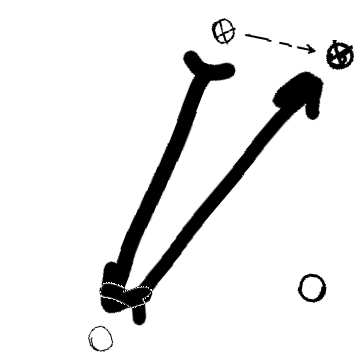
\includegraphics[width=0.92\textwidth]{images/2_0.png}}
    \end{subfigure}
    \begin{subfigure}[b]{0.19\textwidth}
        \fbox{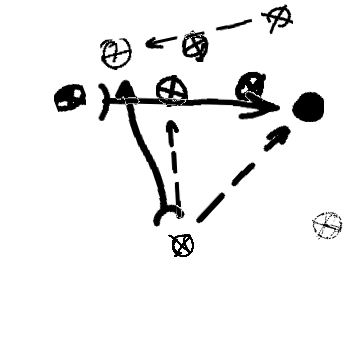
\includegraphics[width=0.92\textwidth]{images/2_1.png}}
    \end{subfigure}
    \begin{subfigure}[b]{0.19\textwidth}
        \fbox{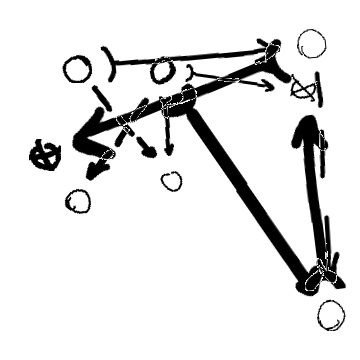
\includegraphics[width=0.92\textwidth]{images/2_2.png}}
    \end{subfigure}
    \begin{subfigure}[b]{0.19\textwidth}
        \fbox{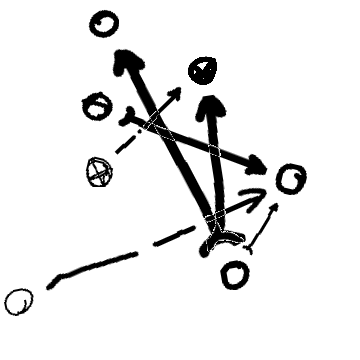
\includegraphics[width=0.92\textwidth]{images/2_3.png}}
    \end{subfigure}
    \begin{subfigure}[b]{0.19\textwidth}
        \fbox{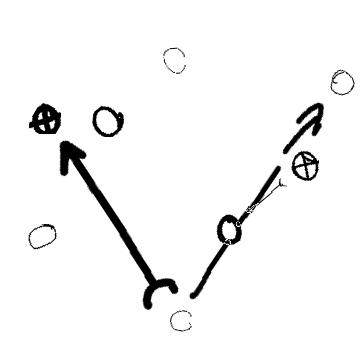
\includegraphics[width=0.92\textwidth]{images/2_4.png}}
    \end{subfigure}
    \caption[Randomly connected nodes using constraint data]{Samples of images generated by connecting randomly selected pairs of nodes using the prepared constraint data. Please note that the colors of these samples are inverted.}\label{fig:constraint_data_step2}
\end{figure}

\subsubsection{Cropping images to get the training data}\label{ch:cropping_images}

At last, these images are cropped.
By cropping and reshaping the models the images can be fed into the training process of a Keras model.
The notebook doing this operation can be viewed at \url{https://aka.klawr.de/sep\#4}.
As the number of possible connections is \(34 = \frac{\sum_{i=3}^{9}i(i-1)}{(10-3)}\), the expected number of generated crop-images is 3.400.000.
It is also important to check for reversed constraints between node pairs to classify them as a non-connection, to be able to correctly predict the direction of the constraint, too.
As 100.000 images are already a good size to work with, another measure was taken to keep the number of expected crops in check.
For this crops are only kept \(\frac{1}{m(m-1)}\) of the time, which is about each 30th time in this case.

The resulting dataset contains 119.189 images, which are subsequently transformed into a \name{tensorflow record}.

% TODO image of the crops here...

With the data prepared the next step is to train the constraint detecting model.

\subsubsection{Training of the constraint detection model}

In this prototype, the design of the constraint detection model is a copy of the results of the previously trained symbol detector.
The input size is adapted to fit for the crops, which have a size of 96 by 96 instead of the 32 by 32 images used for the symbol detector.
The model is created using the functional API of Keras, which has no real impact on the result, but is just another way of defining models.

The output of \code{model.summary()} can be viewed in Listing~\ref{lst:crop_model}.
\begin{lstlisting}[label={lst:crop_model}, caption={Summary of Constraint Detector.}]
Model: "model"
_________________________________________________________________
Layer (type)                 Output Shape              Param #   
=================================================================
input_1 (InputLayer)         [(None, 96, 96, 1)]       0         
_________________________________________________________________
conv2d (Conv2D)              (None, 96, 96, 16)        272       
_________________________________________________________________
max_pooling2d (MaxPooling2D) (None, 48, 48, 16)        0         
_________________________________________________________________
conv2d_1 (Conv2D)            (None, 48, 48, 32)        8224      
_________________________________________________________________
max_pooling2d_1 (MaxPooling2 (None, 24, 24, 32)        0         
_________________________________________________________________
flatten (Flatten)            (None, 18432)             0         
_________________________________________________________________
dense (Dense)                (None, 3)                 55299     
=================================================================
Total params: 63,795
Trainable params: 63,795
Non-trainable params: 0
_________________________________________________________________    
\end{lstlisting}

The training is done by decoding the record which was created in earlier steps and then splitting the data into 80.000 images for training, 20.000 images for validation, and the remaining 19.189 images are used for testing the model.

The training is then initiated by using the \code{model.fit} method, passing the training data as the arguments.
\name{TensorBoard} % TODO citation needed
is used to log the accuracy and the loss of the model during training.
The respective graphs can be seen in figure~\ref{fig:crop_detector_tensorboard}.

\begin{figure}
    \centering
    \begin{subfigure}[b]{0.45\textwidth}
        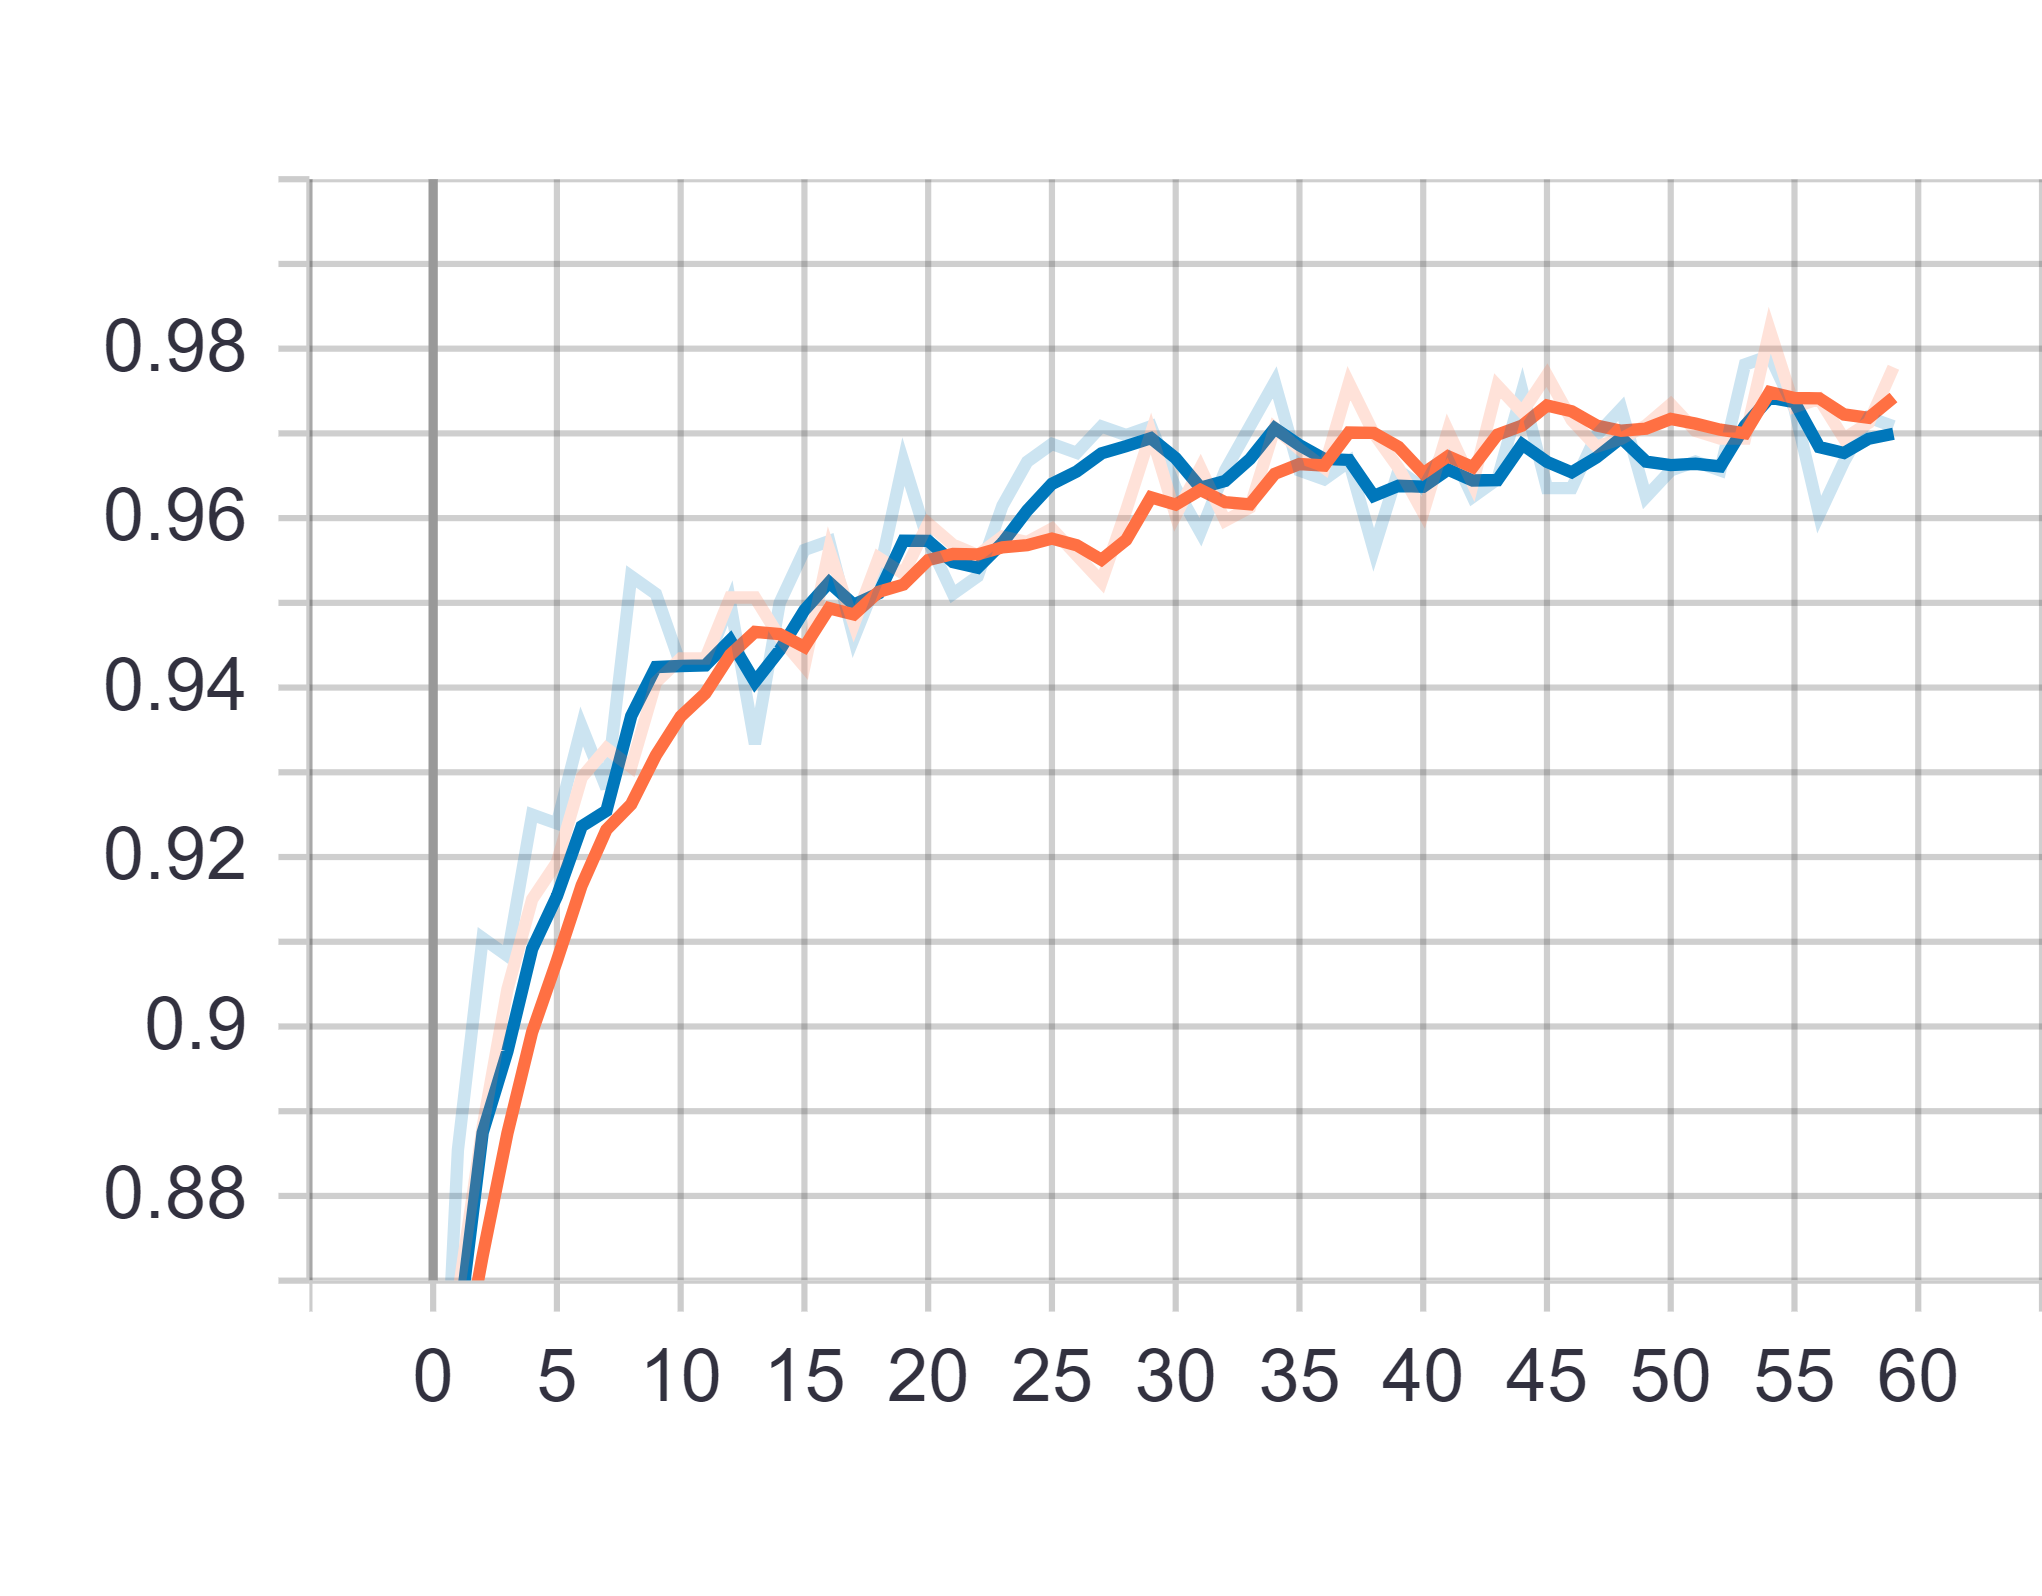
\includegraphics[width=\textwidth]{images/crop_detector_epoch_acc.png}
    \end{subfigure}
    \begin{subfigure}[b]{0.45\textwidth}
        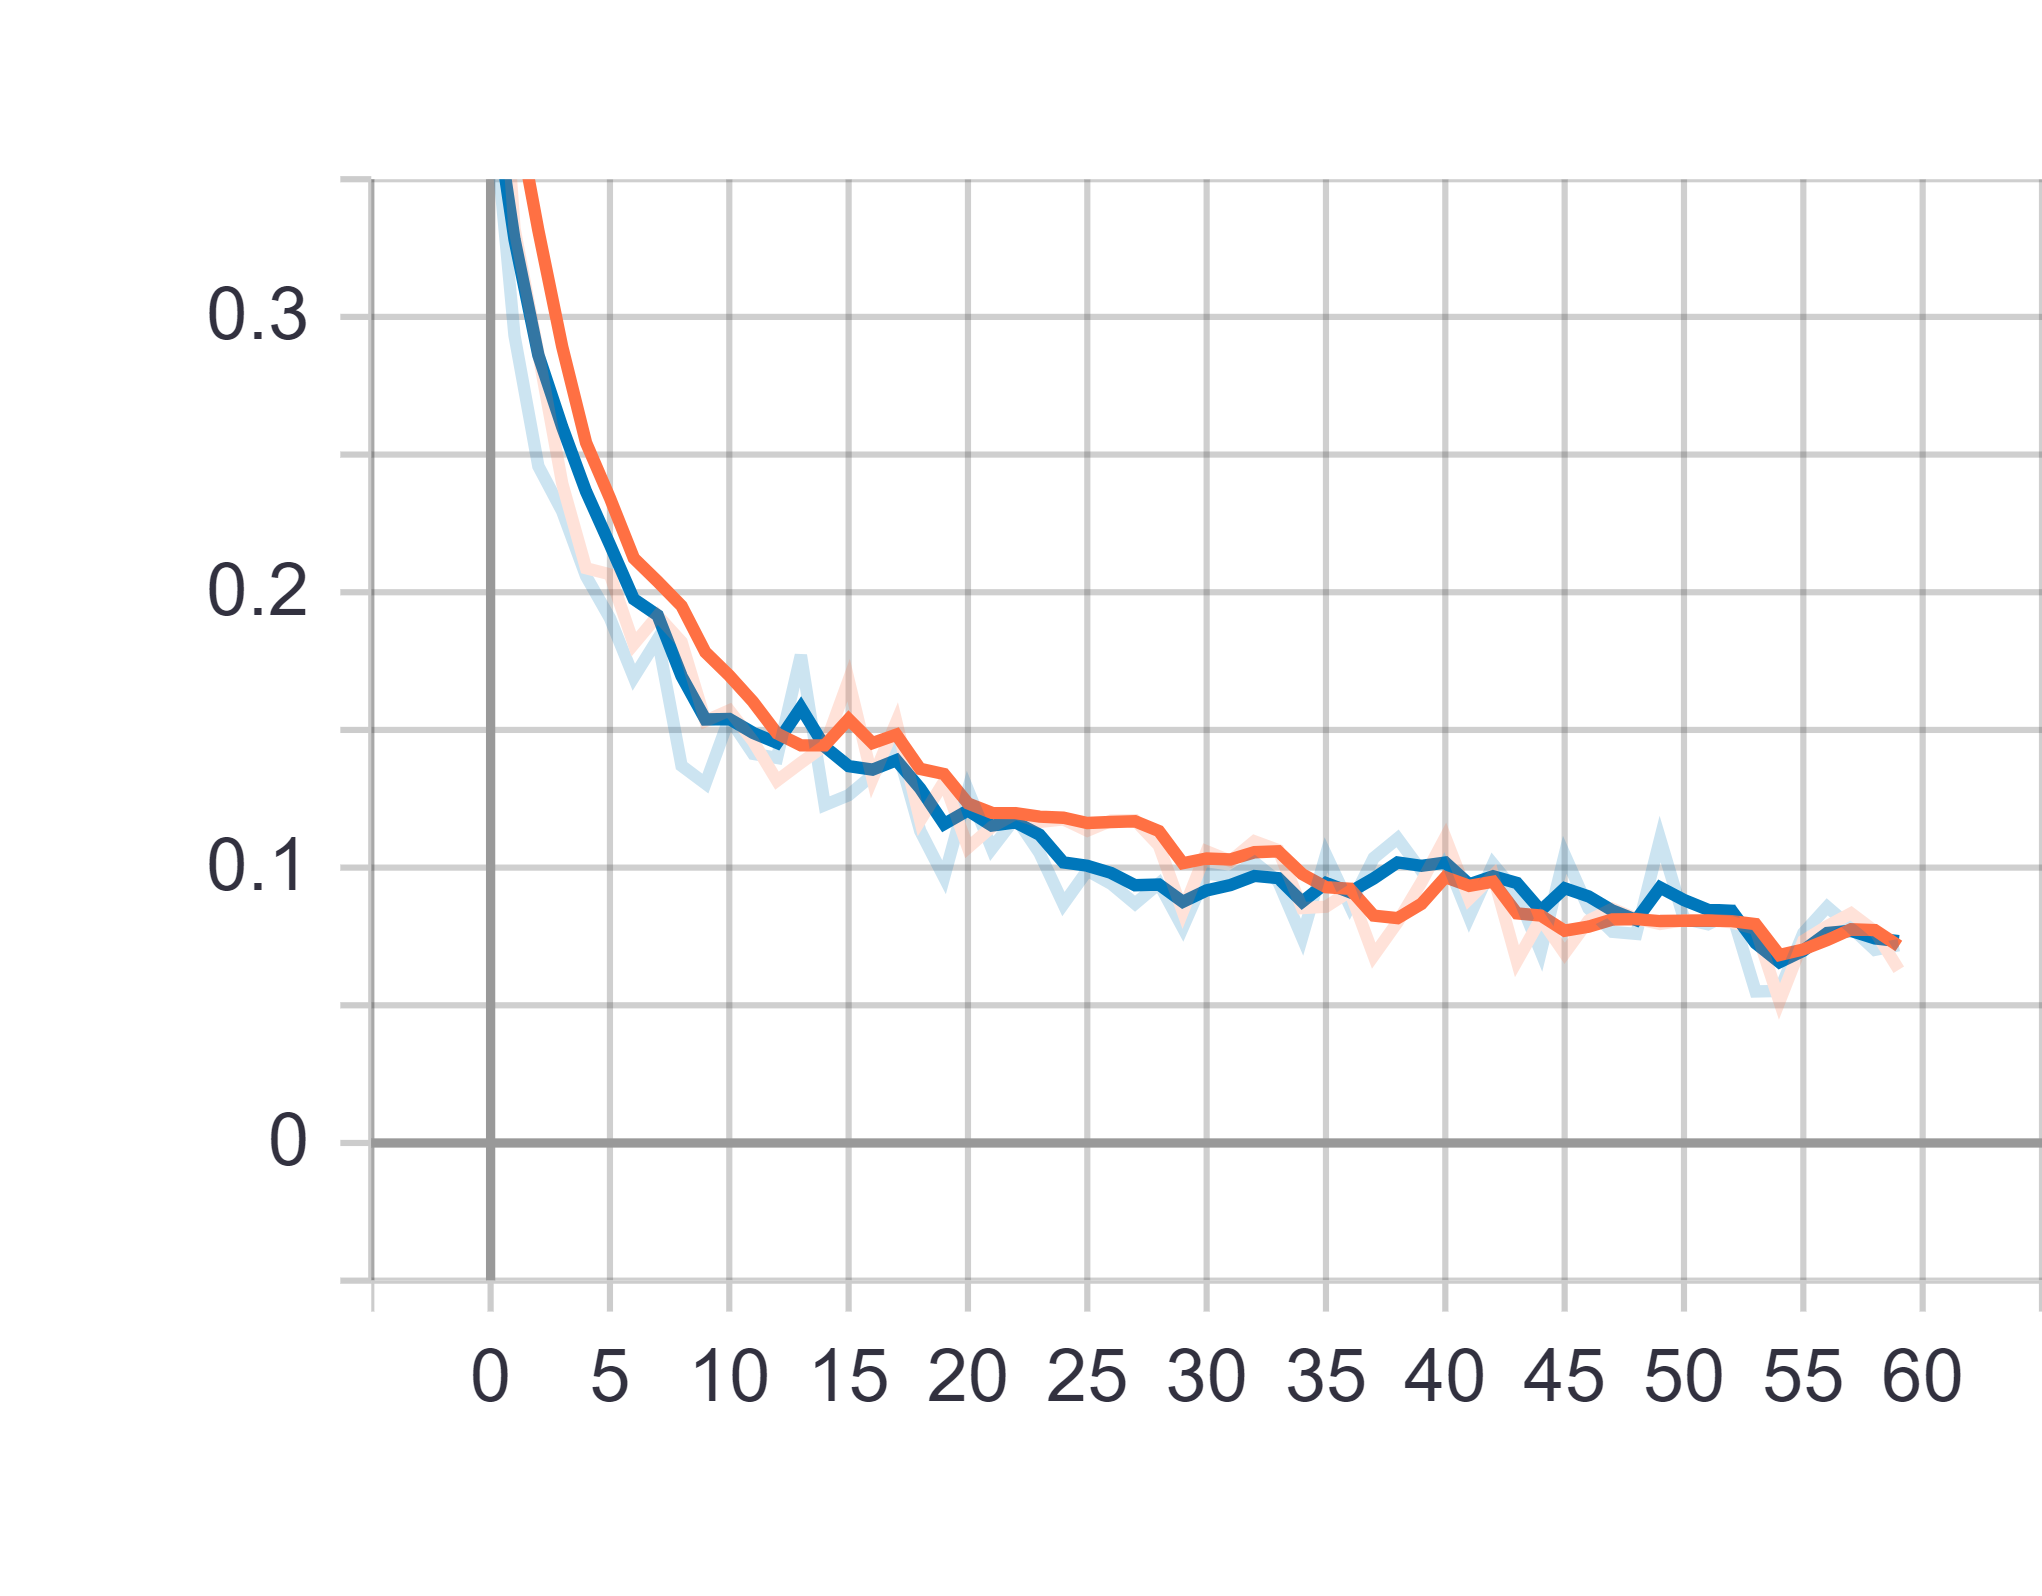
\includegraphics[width=\textwidth]{images/crop_detector_epoch_loss.png}
    \end{subfigure}
    \caption[TensorBoard output for the crop detector]{The training accuracy and loss of the crop detector. These graphs were created using TensorBoard, which is used as the callback during training.}\label{fig:crop_detector_tensorboard}
\end{figure}

\subsubsection{Combining node and constraint detection}

To be able to predict constraints in production the generation of crops has to be implemented as an intermediate step between the node and constraint detection.
The images must be cropped according to the generation of the training data, which means the coordinates of the nodes have to be detected first, and the area between them is resized to 96 by 96 images.
Previously the nodes are placed on the image using (randomly) given coordinates.
This process is now revered, getting the coordinates using the Fully Connected Network on the training data and processing the data.

The constraint detection relies heavily on the performance of the node detection because nodes that are not detected are not taken into account when creating the data for the constraint detector.
Falsely predicted nodes are most likely not going to result in a pair of nodes connected by constraints, since the resulting crop would most likely not look like a constraint, but they are slowing the process down significantly since the number of crops grows exponentially to the number of nodes.

A pipeline of this process can be reviewed at \url{https://aka.klawr.de\#5}.

\begin{figure}
    \centering
    \begin{subfigure}[b]{0.19\textwidth}
        \fbox{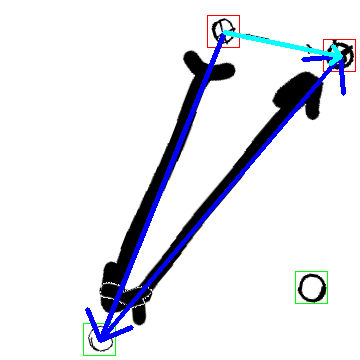
\includegraphics[width=0.92\textwidth]{images/225_0rc.png}}
    \end{subfigure}
    \begin{subfigure}[b]{0.19\textwidth}
        \fbox{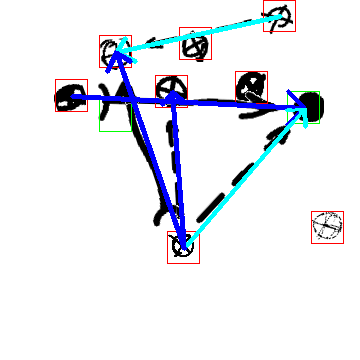
\includegraphics[width=0.92\textwidth]{images/225_1rc.png}}
    \end{subfigure}
    \begin{subfigure}[b]{0.19\textwidth}
        \fbox{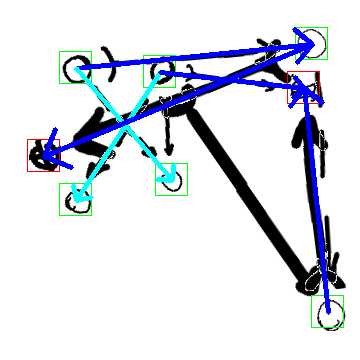
\includegraphics[width=0.92\textwidth]{images/225_2rc.png}}
    \end{subfigure}
    \begin{subfigure}[b]{0.19\textwidth}
        \fbox{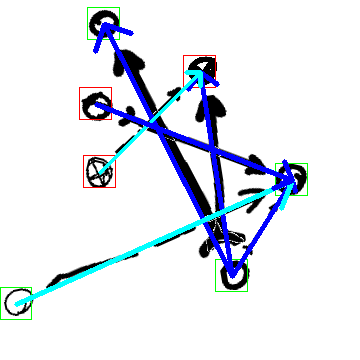
\includegraphics[width=0.92\textwidth]{images/225_3rc.png}}
    \end{subfigure}
    \begin{subfigure}[b]{0.19\textwidth}
        \fbox{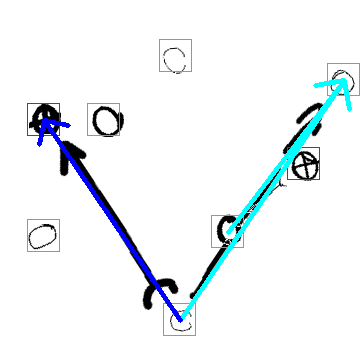
\includegraphics[width=0.92\textwidth]{images/225_4rc.png}}
    \end{subfigure}
    \caption[Predictions of the first prototype on the generated data]{The second step of the data generation processed created images with nodes and constraints that resemble nodes and constraints placed randomly into a canvas. These predictions are made on the images from figure~\ref{fig:constraint_data_step2}. There is only one falsely predicted node in the second image from the left. The constraints are way less accurate, which is not surprising considering the composition of these images.}\label{fig:constraint_data_step3}
\end{figure}

\subsection{Conversion to the web context}\label{ch:conversion_to_web_context}

So far all the code is written in Python.
To make the data pipeline available in a web-based context, the models have to be converted into a format readable by JavaScript and the pipeline has to be adjusted accordingly.

For the conversion of the models, the library \name{Tensorflow.js} % TODO citation needed
is used.
\name{Tensorflow.js} takes the model file as input and outputs a description of the model in \name{JSON} format.
The trained weights and biases are contained in \name{group1-shard1of1.bin}\footnote{Instructions on how to import a Keras model into Tensorflow.js can be viewed at \url{https://aka.klawr.de/sep\#6}.}. % TODO https://www.tensorflow.org/js/tutorials/conversion/import_keras

To include the weights and biases into an importable JavaScript file it is converted into a base64-formatted string.
For this the \name{base64}~\cite{Josefsson2018} module contained in \name{GNU Coreutils} is used.
The resulting string is copied into a JavaScript file, containing one class, as can be seen in Listing~\ref{lst:js_model_class}.

\begin{lstlisting}[label={lst:js_model_class}, caption={[JavaScript classes for Tensorflow.js.] Class definition of one of the models providing necessary functions to be used by \code{tf.loadLayersModel} to return a usable model in JavaScript. }]
class ConstraintModel {
    model=`{/* JSON with information about the model */ }`;
    bin=`/* base64 string with information about weights and biases */`;
    async load() {
        function base64Decode(base64) {
            const binaryString = window.atob(base64);
            const bytes = new Uint8Array(binaryString.length);
            for (let i = 0; i < binaryString.length; ++i) {
                bytes[i] = binaryString.charCodeAt(i);
            }
            return bytes.buffer;
        }
    
        const a = JSON.parse(this.model);
        a.weightSpecs = a.weightsManifest[0].weights;
        a.weightData = base64Decode(this.bin);
        return a;
    }
}
\end{lstlisting}

The contents of some properties are commented out, to keep this listing concise.
The full file can be reviewed at \url{https://aka.klawr.de/sep\#7}. % TODO https://raw.githubusercontent.com/klawr/deepmech/wip/sep/reports/sep/code/old/crop.js but in the master branch of course.

For the conversion, each model is assigned to one class, which has three properties.
\code{model} contains the content of the JSON and \code{bin} the base64-string without any further modifications.
Furthermore, objects created by this class contain a \code{load} function, which returns the respective model by parsing the JSON into an object, where the \code{weightData} of the model is added by decoding the content of \code{bin}.

A model can then be created by issuing \code{tf.loadLayersModel(new Crop())}.

At the moment it is not possible to convert a model into a Tensorflow model after it is processed in any form.
Therefore a function has to be written which takes the initially used node detector as input and converts it into an FCN.\@
For this a generalized form of the conversion processed has been written, which can be reviewed at \url{https://aka.klawr.de/sep\#8}. % TODO

The models are implemented into the JavaScript pipeline by embedding all necessary functions into an object, called \code{deepmech}.
This object has 6 properties, which are used to use the previously defined classes to create models and predict images using them.

\begin{enumerate}
    \item \code{nodeDetector} --- an immediately invoked function execution is used to call the \code{tf.loadLayersModel} function provided by Tensorflow.js by submitting a \code{new models.NodeModel()}.
    The return of this function is immediately used as input for the \code{toFullyConv} function.
    \item \code{constraintDetector} --- a function similar to the \code{nodeDetector} property, but without the necessity to convert the model into a FCN.\@
    \item \code{detectNodes} --- this function takes an image and the previously defined nodeDetector as input and returns the detected nodes with some preprocessing steps in between.
    \item \code{getCrops} --- another function which uses an image and previously determined nodes to create crops. These crops are equivalent to those generated in Chapter~\ref{ch:cropping_images}.
    \item \code{detectConstraints} --- The generated crops are used in conjunction with the model returned by \code{constraintDetector} to predict constraints.
    \item \code{predict} --- This function is intended to be used by external processes.
    It combines all other functions by taking an image as input and returning the respective predictions of nodes and constraints in an image.
\end{enumerate}

By converting all the necessary steps into a JavaScript pipeline, the \code{deepmech} object may be implemented into a library to be used in any combination.
For demonstration purposes, it is implemented into Node.js % TODO
and by using \name{ijavascript} and the \name{conda} package of Node.js % TODO
integrated into a Jupyter Notebook, which can be viewed at \url{https://aka.klawr.de/sep\#9}.

\subsection{Implementation into mec2}

\subsubsection{mec2}

% TODO this is a 1 on 1 copy from the wiki:
mec2 is a 2D physics simulation engine written in JavaScript.
It is designed to easily create 2D mechanisms for rapid sketching and rendering the resulting models in a 2D canvas using g2.

Mechanisms are defined by using JSON formatting, as shown in Listing~\ref{lst:mec2_example}.

\begin{lstlisting}[label={lst:mec2_example}, caption={ Example for a mechanism defined in the syntax proposed by \name{mec2}. }]
{
    "nodes": [
        { "id": "A0", "x": 75, "y": 50, "base": true },
        { "id": "A", "x": 75, "y": 100 },
        { "id": "B", "x": 275, "y": 170 },
        { "id": "B0", "x": 275, "y": 50, "base": true },
        { "id": "C", "x": 125, "y": 175 } ],
    "constraints": [
        {   "id": "a", "p1": "A0", "p2": "A", "len": { "type":"const" },
            "ori": { "type": "drive", "Dt": 2, "Dw": 6.28 } },
        {   "id": "b", "p1": "A", "p2": "B", "len": { "type":"const" } },
        {   "id": "c", "p1": "B0", "p2": "B", "len": { "type":"const" } },
        {   "id": "d", "p1": "B", "p2": "C", "len": { "type":"const" },
            "ori": { "ref": "b", "type": "const" } } ],
    "views": [
        {   "show": "pos", "of": "C", "as": "trace", "Dt":2.1,
            "mode":"preview", "fill":"orange" },
        {   "show": "vel", "of": "C", "as": "vector" },
        {   "as": "chart", "x": 340, "y": 75, "Dt": 1.9,
            "show": "wt", "of": "b" } ]
}
\end{lstlisting}

\begin{figure}
    \centering
    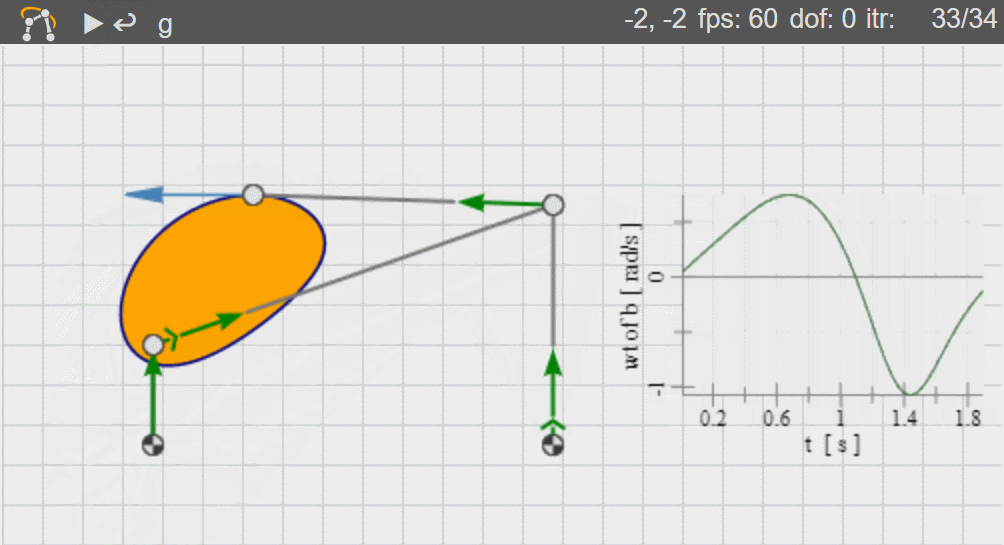
\includegraphics[width=0.8\textwidth]{images/mec2_chart.png}
    \caption[Example of the mec2 HTML element]{ The mechanism defined in Listing~\ref{lst:mec2_example}. It is rendered using the mec2 custom HTML element. Defined are five nodes and 4 constraints. The chart and trace views are generated after one revolution of the leftmost constraint. }\label{fig:generated_data_samples}
\end{figure}

mec2 is divided into many sub-modules; some of which are optional, but some are necessary to simulate functioning mechanisms.

For this prototype only necessary modules have to be used; namely:
% TODO fill this a bit more:
\begin{enumerate}
    \item \name{mec2.core}, which defines the central JavaScript object other modules are built upon.
    The core \code{mec} object defines central properties, which make it easy to change certain parameters for the whole simulation.
    Tolerances are defined for exit conditions inside the iterative calculations of the simulation.
    Central settings for rendering, such as colors for individual parts, color modes for readability in light and dark environments are defined here.
    To show and hide certain parts of the mechanism can be controlled here.
    For each of these properties default values are set.

    \item \name{mec2.model} adds certain functionality to the \code{core} object. 
    This and other \name{mec2} modules add properties to the prototype of the \name{mec2} core object.
    \code{models} \code{extend} function sets the prototype of a JavaScript object to be the prototype of \name{mec2}'s \code{core} Object.
    This approach allows for easy extensibility of objects by adding modules to the core object.

    \name{mec2.model} also serves as a hub for all other modules to be implemented in.
    By delegating certain functionality it suffices to issue e.g.\ the model's \code{init} function to call \code{init} on all other objects handled by other modules as well.
    
    \item \name{mec2.node} implements one of the two essential elements of mechanisms (the other being constraints). Nodes are to be seen as particles, which can have a degree of freedom of 2. They are implemented with a default mass of 1kg.
    
    Nodes do not interact with anything but the environment, so no collision is implemented.
    They are only restricted in certain movements by constraints.

    \item \name{mec2.constraint}s are the only thing able to restrict nodes in certain directions.
    Usually a constraint is used to reduce the degree of freedom of a node by one, but it is also possible to take all two degrees of freedom of a node, or none.
\end{enumerate}

At the time of writing five other modules\footnote{The other modules being \name{mec2.load}, \name{mec2.drive}, \name{mec2.view}, \name{mec2.msg.en} and \name{mec2.shape}} % TODO is this footnote relevant?
exist to extend the functionality of \name{mec2}, but they do not concern the implementation of \name{deepmech} and are not further discussed here.

Additionally \name{mec2} provides a custom HTML element, which allows for an easy implementation into web pages.
The object defining the model is given as JSON inside the \code{innerHTML} of the respective custom HTML to define the input, which is respectively parsed using the built-in function \code{JSON.parse()}. % TODO
The custom HTML element adds other functionality besides the appropriate implementation of \name{mec2} with all modules.

\subsubsection{g2}

For rendering models \name{g2} is used. % TODO cite
\name{g2} is a JavaScript library that constructs an array of commands which can then be handed over into a drawing context via a dedicated \code{exe} method.
The default handler of \name{g2} issues commands to a canvas handler, which in turn uses the standard built-in canvas API to draw images on an HTML canvas element.

\begin{wrapfigure}{r}{0.35\textwidth}
    \centering
    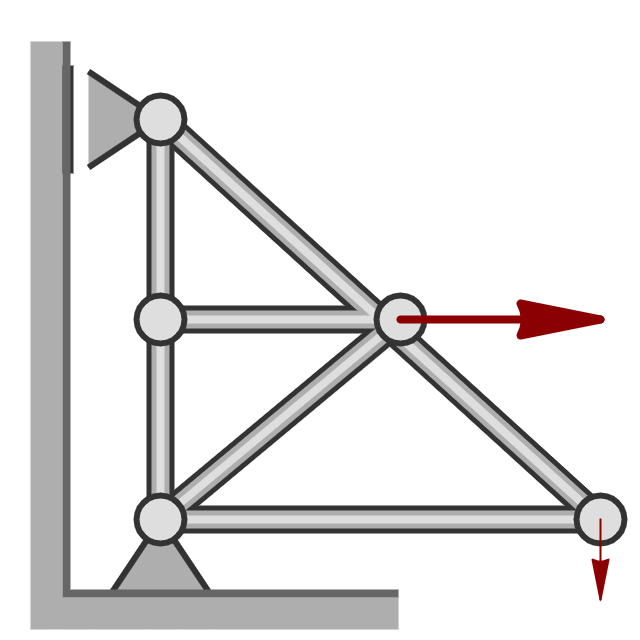
\includegraphics[width=0.35\textwidth]{images/truss.png}
    \caption{Image generated by Listing~\ref{lst:truss}.}\label{fig:truss}
\end{wrapfigure}

\begin{lstlisting}[label={lst:truss}, caption={Example code of a truss defined with g2.}]
const A = { x: 40, y: 30 },
    B = { x: 150, y: 30 }, C = { x: 40, y: 80 },
    D = { x: 100, y: 80 }, E = { x: 40, y:130 };

g2().view({ cartesian: true })
    .link2({ pts: [ A, B, E, A, D, C ]})
    .nodfix({ ...A, scl: 1.5 })
    .nodflt({ ...E, scl: 1.5, w: -Math.PI / 2 })
    .nod({ ...B, scl: 1.5 })
    .nod({ ...C, scl: 1.5 })
    .nod({ ...D, scl: 1.5 })
    .vec({
        x1: D.x, y1: D.y, x2: D.x + 50,
        y2: D.y, ls:'darkred', lw :2 })
    .vec({
        x1: B.x, y1: B.y, y2: B.y - 20,
        x2: B.x, ls:'darkred', lw :0.5 })
    .ground({ pts: [
        { y: E.y + 20, x: E.x - 23 },
        { y: A.y - 18, x: A.x - 23 },
        { y: A.y - 18, x: D.x }]})
    .exe(ctx)
\end{lstlisting}

Likewise \name{mec2}, \name{g2} is structured in a modular manner, but the \name{g2.core} module suffices for basic drawings.
At the time of writing six other modules exist for \name{g2}\footnote{Namely \name{g2.ext}, \name{g2.lib}, \name{g2.io}, \name{g2.mec}, \name{g2.chart}, \name{g2.selector} and \name{g2.editor}.}, but at this point only the modules relevant to the case will be examined more closely.

\name{g2.ext} provides the necessary functionality for other modules to use, such as positioning capability for labels.
Modules like \name{g2.chart} provide only one new (but extensive) command, which can be subsequently used by other libraries, like \name{mec2}.
\name{g2.mec} provides definitions to draw shapes and symbols that are often used in engineering, as can be seen in figure~\ref{fig:truss}.
\name{g2.selector} is an extension used in interactive environments to be able to select certain geometries and interact with them.
For this purpose \name{g2.selector} enables the introduction of a new context which can be used to find elements whose coordinates match those of a corresponding mouse pointer.

\subsubsection{canvasInteractor}

The \name{canvasInteractor.js} % TODO
is an interaction manager for the HTML canvas element.
It is used to centralize all interactions and animation requests.
\code{canvasInteractor} manages one \code{requestAnimationFrame}, which minimizes overhead as if each component would issue a new request.
Additionally, this approach parallelizes all requests, because they are all handled in one function call.

New \code{instances} can be added to the \code{canvasInteractor} object by calling its \code{add} function, but to create a new interactor the \code{create} function has to be issued, which applies the prototype of the \code{canvasInteractor} object onto the variable.
The created objects get all event listeners necessary to provide the full capability for interactions.

\subsubsection{Putting it together}

% TODO add some subsubsections.

The next step is to implement \name{deepmech} into this set of libraries.
At first a script is written, which adds the necessary functionality into all \name{mec2} HTML elements.
This is done by \code{document.getElementsByTagName('mec-2')} and then iterating over the returned array, to ensure the extensions are applied everywhere.

The target of the written script is to create the possibility inside the \name{mec2} HTML element to create images, predict nodes and constraints and return the respective \name{mec2} representation.

For the activation of the additions described here a button has been added to the navigation bar.
The respective button in the form of a pencil can bee seen in figure~\ref{fig:prototype_before}.
The activation of the button initiates a few changes to the navigation bar, which changes the context the user interacts with, which can be seen in the navigation bar in figure~\ref{fig:prototype_drawing}.

\begin{figure}
    \centering
    \begin{subfigure}[b]{0.32\textwidth}
        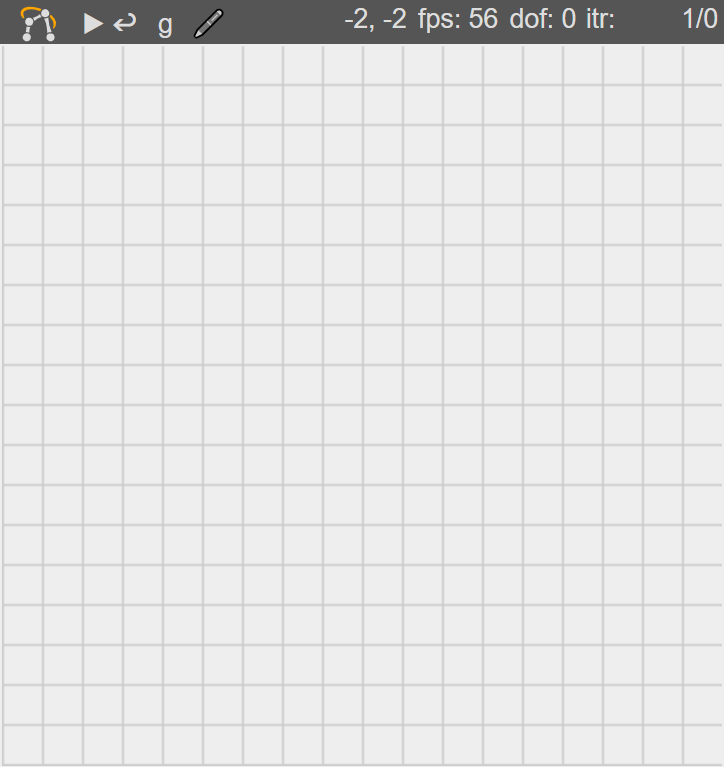
\includegraphics[width=\textwidth]{images/prototype_before.png}
        \caption{}\label{fig:prototype_before}
    \end{subfigure}
    \begin{subfigure}[b]{0.32\textwidth}
        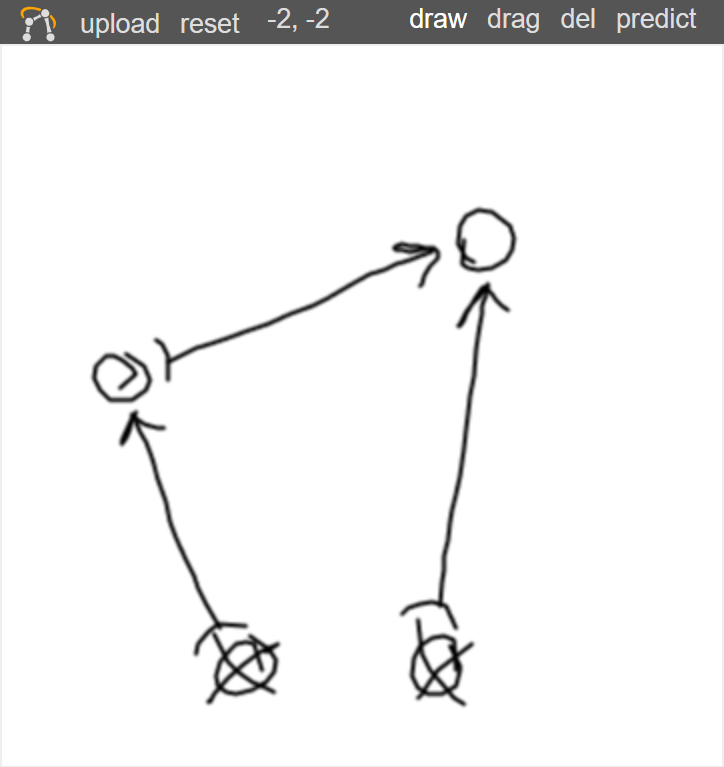
\includegraphics[width=\textwidth]{images/prototype_drawing_inverted.png}
        \caption{}\label{fig:prototype_drawing}
    \end{subfigure}
    \begin{subfigure}[b]{0.32\textwidth}
        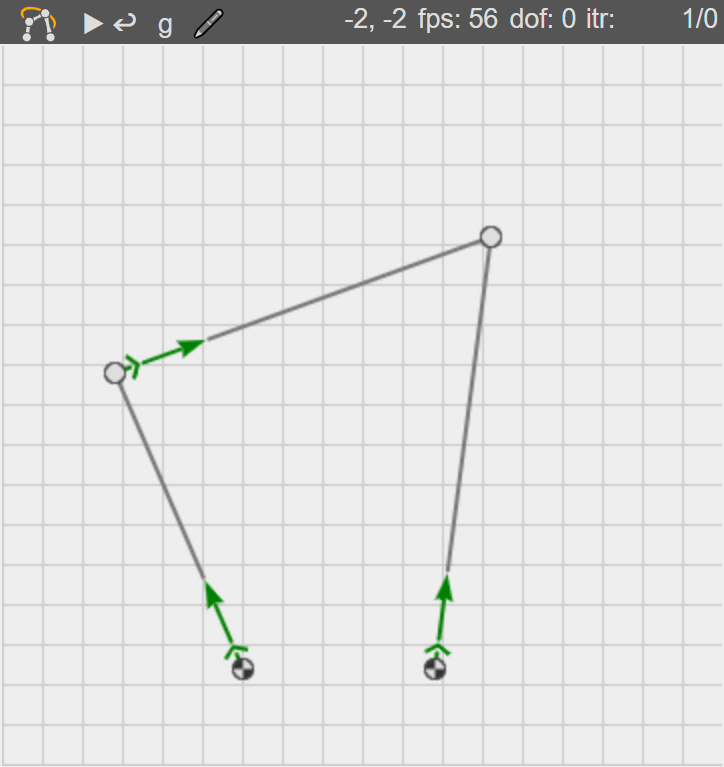
\includegraphics[width=\textwidth]{images/prototype_after.png}
        \caption{}\label{fig:prototype_after}
    \end{subfigure}
    \caption[deepmech prototype.]{The first image depicts \name{mec2} in its default state. The only thing visible due to the additions is the pencil symbol in the navigation bar.
    The second image depicts a drawing of a four-bar. Please note that the actual image is inverted, but that does not make any real difference.
    The third image shows the predicted mechanism.}\label{fig:prototype}
\end{figure}

Changes in the canvas are managed by only one \name{g2} command queue, which inherits multiple other command queues for each different case, as can be seen in Listing~\ref{lst:prototype_command_queue}.

\begin{lstlisting}[caption={Command queue for the drawing context in the prototype.}, label={lst:prototype_command_queue}]
const command_queue = g2().rec({
        x: () => -view.x / view.scl,
        y: () => -view.y / view.scl,
        b: () => element.width / view.scl + 1,
        h: () => element.height / view.scl + 1,
        fs: '#000',
        isSolid: false
    })
    .view(view)
    .use({ grp: () => img_placeholder })
    .use({ grp: () => mec_placeholder })
    .use({ grp: () => ply_placeholder });
\end{lstlisting}

Herein \code{view} is taken from \code{element.\_interactor.view} of the respectve \name{mec2} \code{element}.

The background of the drawing canvas is colored black (\code{\#000}) by issuing the \code{rec} command of \name{g2} for the active viewport\footnote{Please note that figure~\ref{fig:prototype_drawing} contains an inverted image for contrast reasons.}.

The \code{img\_placeholder} is used to draw images loaded by issuing \code{uploadImage}, which loads an image and saves the respective image inside this command queue.

The \code{mec\_placeholder} is used to be able to show already determined nodes and constraints of the mechanism inside the drawing context.
This makes it possible to extend existing mechanisms.
A \name{mec2} model is usually defined by more than just nodes and costraints, so all elements which are not part of code{element.\_model.nodes} or \code{element.\_model.constraints} are filtered first; e.g.\ the chart which can be seen in figure~\ref{fig:generated_data_samples}.

The \code{ply\_placeholder} is responsible for rendering user-generated drawing.
The default behavior of the \name{canvasInteractor} when pressing the pointer-button in combination with movement of the pointer is to drag the viewport, or, when an element is selected by the \name{g2.selector}, to drag an element.
When the drawing mode is active this behavior has to be replaced.
When the draw mode is active and \code{pointerdown} is issued an array is created which is then filled by the coordinates of the pointer on each \code{tick}\footnote{A \code{tick} is issued by the \name{canvasInteractor} on each requestAnimationFrame}.
This approach creates one \code{ply} element for each consecutive line, which can be dragged or deleted by changing the respective mode using the  \name{g2.selector}.

By starting a prediction the content of the canvas is fed into the trained models, as discussed in Chapter~\ref{ch:conversion_to_web_context}.
The resulting prediction updates the \name{mec2} model.
This is similar to the generation of bounding boxes, but instead of drawing them onto the canvas to show the results, the respective coordinates are added to the \name{mec2} model.
The assembled \name{mec2} model can then be rendered and interacted with.

